
\documentclass[a4paper, 12pt]{article}
\usepackage{graphicx}
\usepackage{float}
\usepackage{listings}
\usepackage{xcolor}

\definecolor{codegreen}{rgb}{0,0.6,0}
\definecolor{codegray}{rgb}{0.5,0.5,0.5}
\definecolor{codepurple}{rgb}{0.58,0,0.82}
\definecolor{backcolour}{rgb}{0.95,0.95,0.92}

\lstdefinestyle{mystyle}{
    backgroundcolor=\color{backcolour},
    commentstyle=\color{codegreen},
    keywordstyle=\color{magenta},
    numberstyle=\tiny\color{codegray},
    stringstyle=\color{codepurple},
    basicstyle=\ttfamily\footnotesize,
    breakatwhitespace=false,
    breaklines=true,
    captionpos=b,
    keepspaces=true,
    numbers=left,
    numbersep=5pt,
    showspaces=false,
    showstringspaces=false,
    showtabs=false,
    tabsize=2
}
\lstset{style=mystyle}


\title{Project assignment in\\
       SSY080, Signals systems and transforms}

\author{Erik Brink, Love Lyckaro}
\begin{document}
\maketitle
\pagenumbering{gobble}
\newpage
\pagenumbering{arabic}

\section*{Question 1}
  \begin{itemize}
    \item The figure below depicts the two plots of ``Action Train 1'':
  \end{itemize}
  \begin{figure}[H]
    \centering
    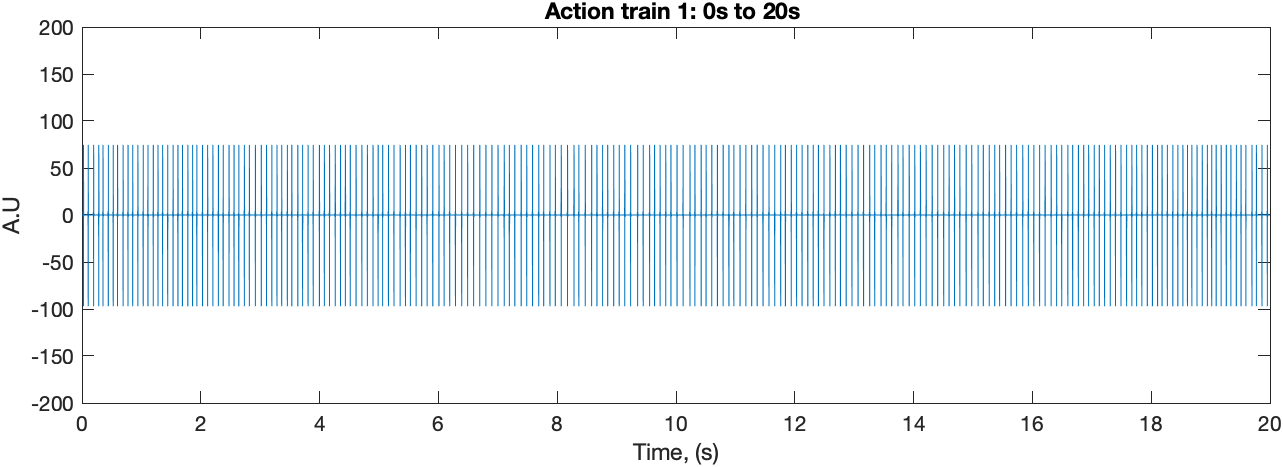
\includegraphics[width= 10cm]{at1_0to20.png}
    \caption{Action train 1 for the full duration of the signal}
  \end{figure}
  \begin{figure}[H]
    \centering
    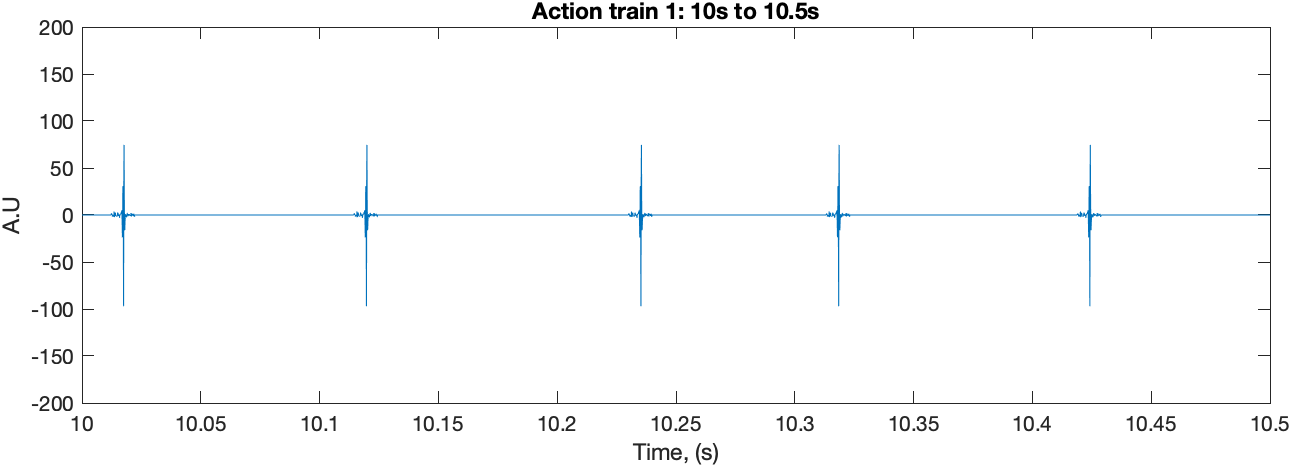
\includegraphics[width= 10cm]{at1_10to105.png}
    \caption{Action train 1 for the interval of 10 s to 10.5 s}
  \end{figure}
  \begin{itemize}
    \item In order to get the action potential trains, we simply need to convelute each \textit{row} of the binary vector with each \textit{row} in the matrix provided by \lstinline{action_potentials.mat} in order to get one train.
    \item The following figure depicts the plot of the EMG-signal in the interval of 10 s to 10.5 s:
  \end{itemize}
  \begin{figure}[H]
    \centering
    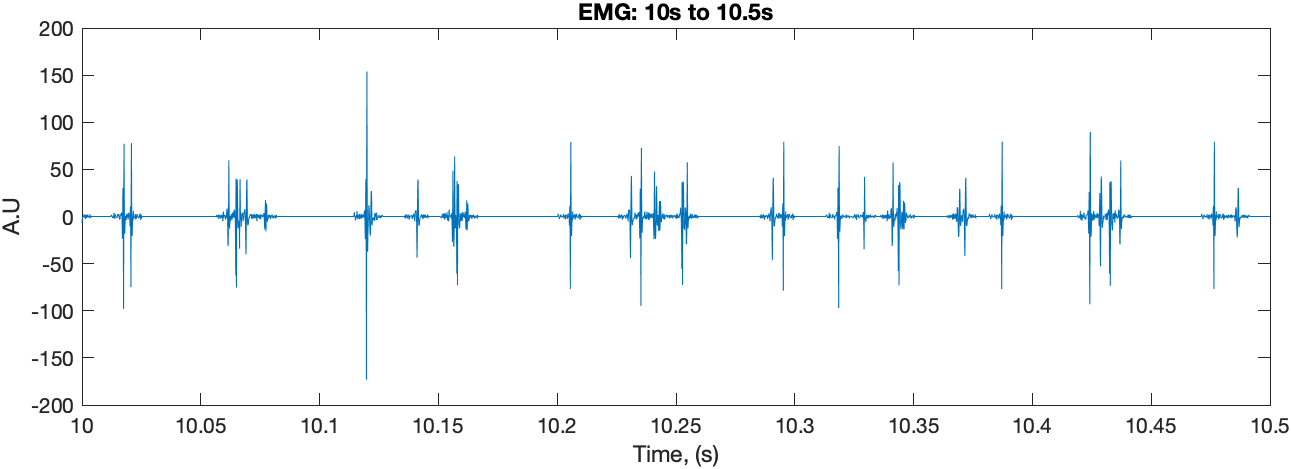
\includegraphics[width= 10cm]{emg_10to105.png}
    \caption{Action train 1 for the interval of 10 s to 10.5 s}
  \end{figure}

\newpage
\section*{Question 2}
  \begin{itemize}
    \item The figure below depicts the plot of the filtered signals as a function of time:
  \end{itemize}
  \begin{figure}[H]
    \centering
    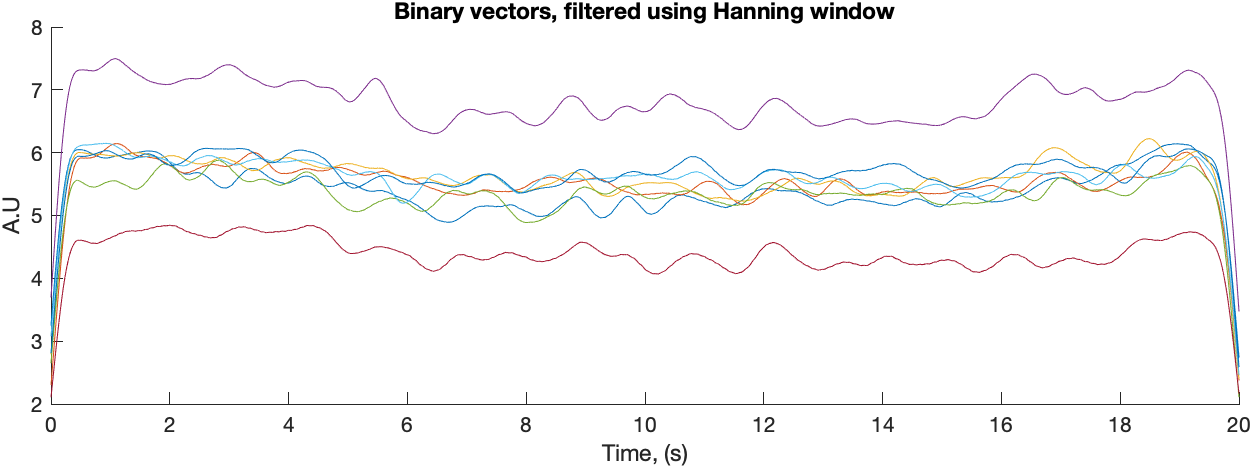
\includegraphics[width= 10cm]{filtered.png}
    \caption{Filtered signals as a function of time}
  \end{figure}
  \begin{itemize}
    \item The characterisrtics of this filter is that of a low-pass filter
  \end{itemize}
\newpage
\pagenumbering{roman}
\section{Code}
    \lstinputlisting[language=Octave]{project.m}
\end{document}
